\setAuthor{}
\setRound{piirkonnavoor}
\setYear{2020}
\setNumber{G 2}
\setDifficulty{2}
\setTopic{TODO}

\prob{Karussell}
Juku läheb lõbustusparki ja märkab tiirlevat karusselli. Karussell koosneb ringikujulisest horisontaalsest kettast, mille küljes ripuvad kettide otsas lõbusõitjad. Juku märkab, et kinnitusketid moodustavad karusselli täiskiirusega pöörlemisel vertikaali suhtes nurga $\theta = \SI{60}{\degree}$.  Leia lõbusõitjate joonkiirus, kui karussell pööreleb täiskiirusel. Mitu tiiru minutis teeb karussell täiskiirusega pööreldes? Karusselli ketta raadius $R=\SI{10}{m}$, kettide pikkus $l=\SI{2}{m}$, raskuskiirendus $g=\SI{9,8}{m / s^2}$. Kettide kaalu mitte arvestada. 


\hint

\solu
Karuselli ketid on pinge all, olgu kettide pinge $T$. Pinget $T$ saab jagada $x$ ja $y$ komponentieks: \pp{1} 
$$T_x=T \cdot \sin{\theta}$$
$$T_y=T \cdot \cos{\theta} \qquad \pp{1} $$
 \begin{center}
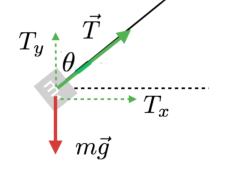
\includegraphics[width=0.3\textwidth]{2020-v2g-02-sol.pdf}
\end{center}
Ketid on horisontaaltasandis ringliikumses, olgu selle joonkiirus $v$. Seega võrdub pinge horisontaalsunnaine projektsioon tsentrifugaaljõuga:
$$T_x = \frac{m v^2}{R_{p}}\quad\quad \pp{1}$$
kus $m$ on Juku mass ja $R_{p} = R + l \cdot \sin{\theta}$ on pöörlemisraadius.
\\
Vertikaalteljes on jõud tasakaalus:
$$T_y=mg \quad \quad \pp{1}$$ 
\\
Asendades $T_x$ ja $T_y$ asemele $T \cdot \sin{\theta}$ ja $T \cdot \cos{\theta}$ ning $R_{p}$, saame võrrandisüsteemi:
$$T \cdot \sin{\theta} = \frac{m v^2}{R + l \cdot \sin{\theta}}$$
$$T \cdot \cos{\theta} = mg \qquad \pp{1}$$ 
\\
Jagades esimese võrrandi teisegas
$$\tan{\theta}= \frac{mv^2}{g(R + l \cdot \sin{\theta})}$$
avaldub lõbusõitja joonkiirus:
$$v= \sqrt{g \cdot \tan{\theta} \cdot (R + l \cdot \sin{\theta})}\approx \SI{14.1}{m/s}. \qquad \pp{1}$$ 
\\
Selleks et leida pöörete arvu minutis, leiame esmalt ühe pöörde aja, ehk perioodi $T$:
$$T=\frac{2 \pi R_{p}}{v}=\frac{2 \pi (R + l \cdot \sin{\theta})}{v}. \qquad \pp{1}$$ 
\\
Seega pöörete arv  $\Delta t = 60\;$s jooksul on
$$N=\frac{\Delta t}{T} =\frac{\Delta t \cdot v}{2 \pi (R + l \cdot \sin{\theta})} \approx \SI{11.5}{}. \qquad \pp{1}$$
\probend